\subsection{Evaluierung} \label{evaluierung}
Damit die Ausarbeitung beginnen kann, muss eine gute Kombination für die zukünftigen Hardware-Komponenten zusammengestellt werden. Diese Kombination sollte auf den Spezifikationen basieren, die vom Projektbetreuer Simon Köldorfer definiert wurden. Diese Spezifikationen umfassen die grundsätzliche Verwendung eines Displays, die IP66-Tauglichkeit des Gehäuses, die Witterungstauglichkeit der Anzeige sowie die Möglichkeit, die Anzeigeseite zu ändern, wobei nicht spezifiziert ist, wie dies umgesetzt werden soll. Die Spannungsversorgung muss außerdem als 24VAC/DC ausgeführt sein. Schließlich sollte die Lösung auch wirtschaftlich sinnvoll sein, falls sich entschieden wird, diese Anzeige fortan an mehreren oder sogar allen Lüftungsgeräten anzubringen. Die genaueren Spezifikationen befinden sich im Kapitel \ref{aufgabenstellung}.\\
Trotz dieser Definitionen blieb genug Freiheit, um mehrere Möglichkeiten zusammenzustellen und somit dem nachzugehen, was für diese Diplomarbeit am passendsten ist. 
Folgend werden alle vier Varianten gelistet, die später auch so innerhalb eines Meetings dem Projektbetreuer näher gebracht wurden. \\
Allgemein zu sagen ist, dass die angegebenen Preise möglicherweise zur Realität etwas abweichen können. Auch, dass die Schwierigkeit der Umsetzungen jeweils bei einem akzeptablen Level liegt und bei allen Varianten die Terminierung oder die Weiterleitung des Modbus-Signals ein Problem sein könnte.
\paragraph{Variante A}
Die erste Variante beinhaltet als einzige den Mikrocontroller Arduino. Genauer gesagt handelt es sich um den Arduino Mega. Unter Abbildung \ref{fig:arduino_mega} findet man eine Darstellugn davon. In dieser Variante war die Grundidee, ein kleines 3.5-Zoll Display mit 1-2 Buttons herzustellen und alles in einer IP66 tauglichen, kleinen Box zu verstauen. 
Die positiven Aspekte dieser Variante beziehen sich sowohl auf den Preis als auch auf die Verfügbarkeit der Teile. Variante A hat mit Abstand den niedrigsten Gesamtpreis, dieser liegt bei ungefähr 63,00 € und die Verfügbarkeit ist stets gegeben. Auch in Bezug auf die Haltbarkeit ist es ein Plus-Punkt, da Witterungen dem Gehäuse nichts ausmachen, und im Falle, dass es doch kaputtgehen würde, es leicht und günstig zu ersetzen ist. Schwierigkeiten existieren jedoch beispielsweise bei der Benutzerfreundlichkeit, da die Bedienung mit 2 Buttons komplizierter bzw. umfangreicher wäre als mit einem. Auch bei den Dokumentationen würde es etwas mangeln, denn während ausreichend über die Hardware zur Verfügung steht, sind die Dokumentationen über die Software bzw. über die Libraries eher kurz gehalten, wie beispielsweise bei der Library \enquote{ModbusMaster}.
\begin{figure}[ht]
	\centering
	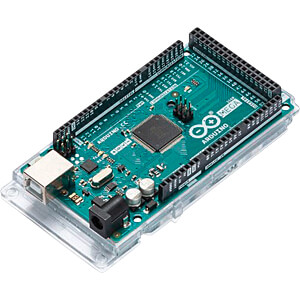
\includegraphics[width=0.5\linewidth]{Bilder/ARDUINO_MEGA.jpg}
	\caption{Arduino Mega (Quelle: \url{https://cdn-reichelt.de/bilder/web/artikel_ws/A300/ARDUINO_MEGA_01_NEU.jpg})}
	\label{fig:arduino_mega}
\end{figure}
\paragraph{Variante B}
Variante B hat als Grundkonzept ein 7-Zoll-Display, welches nicht berührungsempfindlich ist und auch nicht Wasserfest, und deswegen wie in Variante A in eine Witterungsfeste Box gelegt und durch Buttons gesteuert wird. Neben den unterschiedlichen Bildschirmgrößen unterscheidet auch der verwendete Mikrocontroller die beiden Kombinationen, denn hier wird ein Raspberry Pi als Zentralrechner etabliert. Eine Abbildung davon ist in Abbildung \ref{fig:raspi3} zu sehen.\\
Der Gesamtpreis der Hardware liegt bei ungefähr 93.00 € und ist somit auch noch eine der günstigeren Versionen. Für diese Variante sprechen aber noch andere Faktoren. Einerseits die erhöhte Benutzerfreundlichkeit im Vergleich zur Variante A, denn auch wenn wieder Buttons für die Navigation verwendet werden, erleichtert das größere Display die Übersicht. Andererseits die Witterungsfestigkeit aufgrund des Gehäuses, welches bei Schäden leicht und günstig zu ersetzen wäre. Auch Dokumentationen wären ausreichend für Hardware und Software vorhanden. Die Probleme hierbei beziehen sich jedoch auf die Verfügbarkeit des Raspberry Pis, da diese in letzter Zeit entweder wenig verfügbar oder teuer sind. Der Display-Preis ist zwar auch nicht niedrig, kann aber durch Mengenrabatte reduziert werden.
\begin{figure}[ht]
	\centering
	\includegraphics[width=0.6\linewidth]{Bilder/RASPBERRY_PI3.png}
	\caption{Raspberry Pi 3 (Quelle: \url{https://cdn-reichelt.de/bilder/web/xxl_ws/A300/RASPBERRY_PI_3_02_20210420.png})}
	\label{fig:raspi3}
\end{figure}
\paragraph{Variante C}
Die dritte Variante ist die mit Abstand teuerste, denn hier beruht der Preis bei etwa 117,00 €. Der Grund dafür ist, dass die Konzeption aus einem \gls{kapazitiv}n 7-Zoll-Display besteht. Dieses wird unter Abbildung \ref{fig:kapazitives_display} abgebildet. Neben der eigentlich nicht gegebenen Witterungsfestigkeit des Displays per se, würde es jedoch so verbaut werden, dass es dies schlussendlich trotzdem sein sollte. Dennoch könnte sich die Handhabung der Touchfunktion mit der Zeit aufgrund fehlender Wasserdichtigkeit verschlechtern. Da auch hier wieder der Raspberry Pi die Grundlage des Systems spielt, ist auch wieder die Verfügbarkeit dessen ein unpassender Faktor. Positive Aspekte wären allgemein die Touchfunktion, da diese weit verbreitet ist und die Bedienung für den Nutzer einfach hält. Ebenso gibt es ausreichend Dokumentationen für Hardware und Software, trotzdem könnte die Implementation der Touch-Funktion Probleme bereiten.
\begin{figure}[ht]
	\centering
	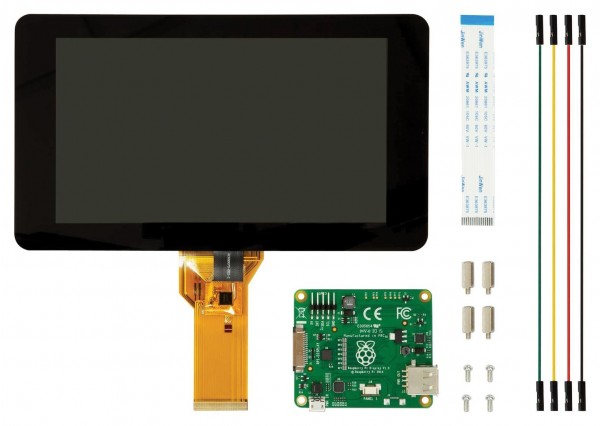
\includegraphics[width=0.6\linewidth]{Bilder/kapazitives_display.jpg}
	\caption{\gls{kapazitiv}s Display (Quelle: \url{https://www.berrybase.at/media/image/49/8e/36/ID_53172_orig_600x600.jpg})}
	\label{fig:kapazitives_display}
\end{figure}
\newpage
\paragraph{Variante D}
Die vierte und letzte Variante charakterisiert sich durch eine weitere Nutzung eines \gls{kapazitiv}n oder diesmal auch \gls{resistiv}n 7-Zoll-Displays, welches nicht wasserdicht ist. Der Zugriff zum Display wird durch eine transparente Klappe am Gehäuse genehmigt. Eine Abbildung dieses Gehäuses befindet sich unter Abbildung \ref{fig:gehäuse_mit_klappe}. Auch hier wird der Raspberry Pi als Mikrocontroller verwendet, welches auf zuvor genannte Probleme bezüglich der Verfügbarkeit zurückführt. Das Display zu erhalten führt zu keinen Schwierigkeiten und man erhält auch wieder einen Mengenrabatt. Nichtsdestotrotz liegt der Gesamtpreis bei ungefähr 108,00 € und ist somit die 2. teuerste Zusammenstellung. Dafür sollten Witterungsprobleme keine Erschwernisse sein, solange nicht vergessen wird, die Klappe am Gehäuse immer ordnungsgemäß zu schließen. Die Situation mit den Dokumentationen ist äquivalent zu Variante B und C und somit auch kein Problem. Zurückkehrend auf die unterschiedlichen Displays: Die \gls{kapazitiv} Version hat eine allgemein besser funktionierende Touch-Funktion, die aber durch nasse Hände genommen wird und somit die Nutzung bei beispielsweise Regen erschwert wird. Die \gls{resistiv} Version ermöglicht dafür besseren Touch mit nassen Händen oder auch Handschuhen.
\begin{figure}[ht]
	\centering
	\includegraphics[width=0.6\linewidth]{Bilder/gehäuse_klappe.png}
	\caption{Gehäuse mit Klappe (Quelle: \url{https://asset.conrad.com/media10/isa/160267/c1/-/de/706888_BB_00_FB/image.jpg?x=1000&y=1000&format=jpg&ex=1000&ey=1000&align=center})}
	\label{fig:gehäuse_mit_klappe}
\end{figure}
\newpage
\paragraph{Bewertungsmatrix}
Um eine klare Übersicht über die potenziell verwendeten Varianten sowie deren spezifische Merkmale zu gewährleisten, wurde eine Bewertungsmatrix in Excel erstellt. Diese Matrix ermöglicht es nicht nur den Teammitgliedern, die sie während eines Meetings präsentieren, die wichtigen Fakten stets im Blick zu behalten, sondern dient auch den Zuhörern als Leitfaden, um die Diskussion besser zu verfolgen. Besagte Matrix befindet sich auf der nächsten Seite unter Abbildung \ref{fig:matrix}.
\begin{landscape}
	\begin{figure}[H]
		\centering
		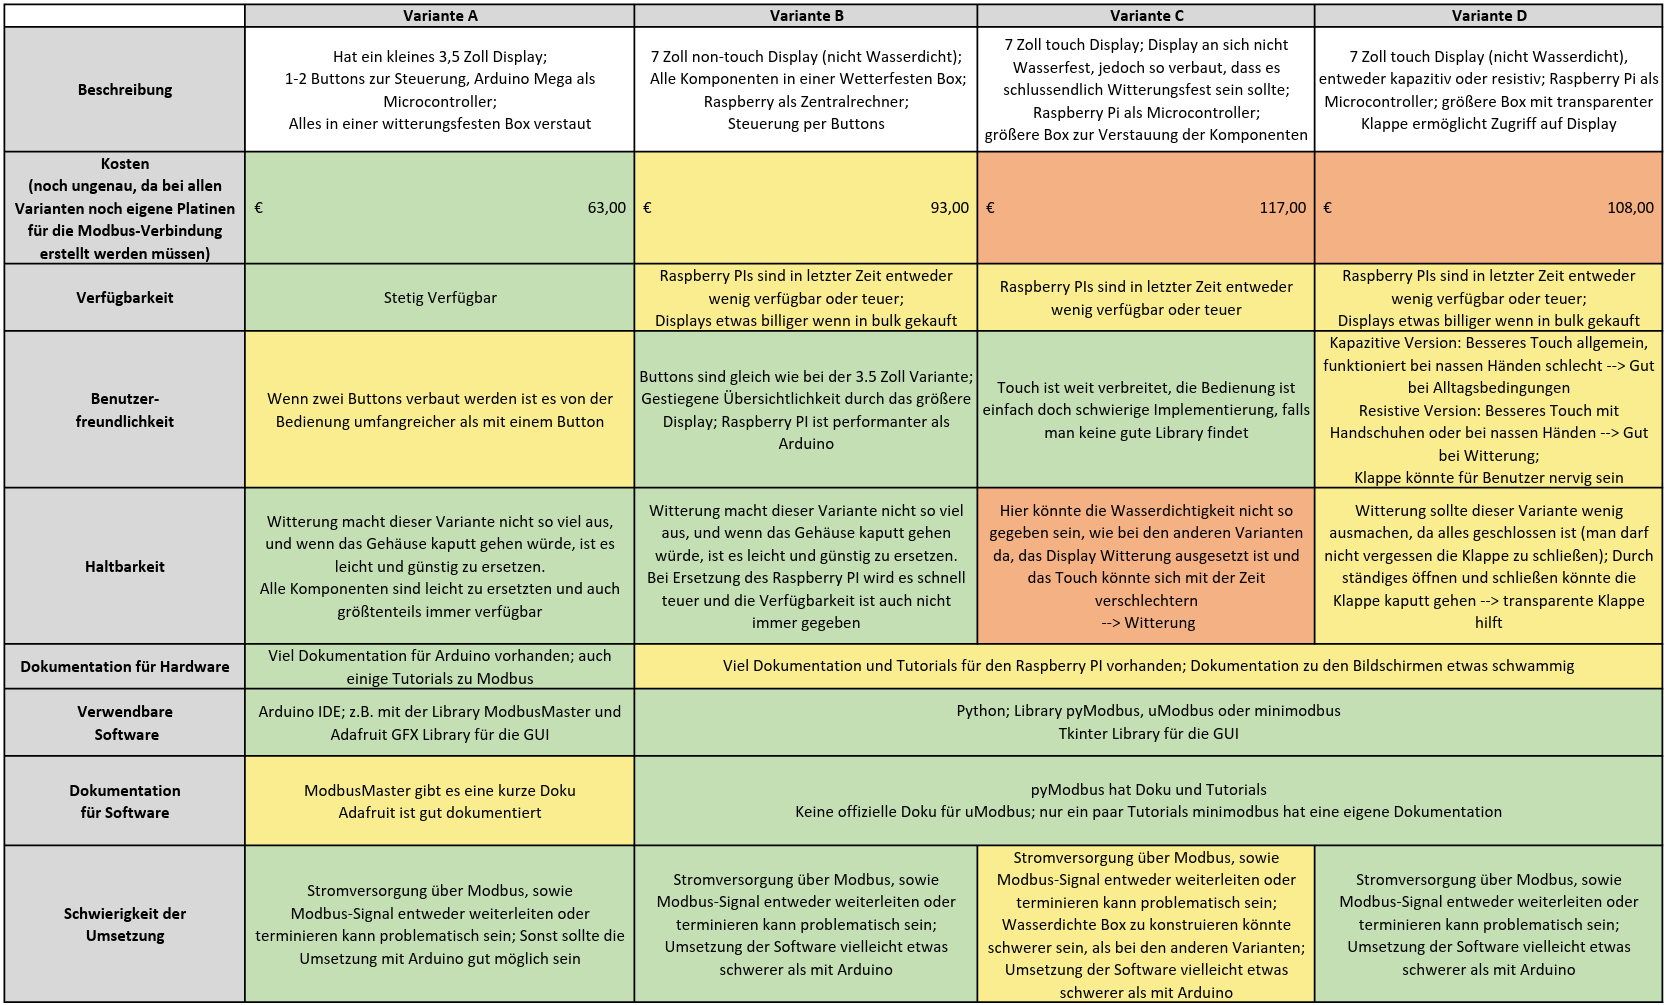
\includegraphics[width=1\linewidth]{Bilder/bewertungsmatrix}
		\caption{Bewertungsmatrix der Hardwarekomponente}
		\label{fig:matrix}
	\end{figure}
\end{landscape}